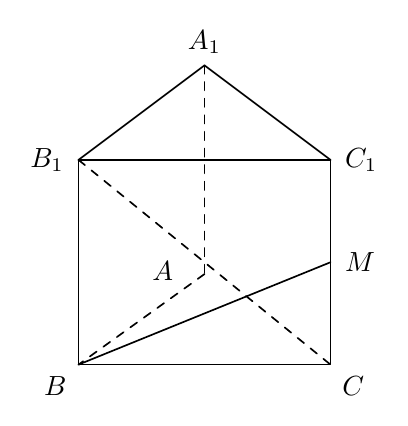
\begin{tikzpicture}[line width=.6pt, line join=round, line cap=round]
% 正三棱柱 ABC-A1B1C1, M 为 CC1 中点
\coordinate (B) at (0,0);
\coordinate (C) at (3.2,0);
\coordinate (B1) at (0,2.6);
\coordinate (C1) at (3.2,2.6);
\coordinate (A1) at (1.6,3.8);
\coordinate (A) at (1.6,1.15);
\coordinate (M) at (3.2,1.3);
% front rectangle
\draw (B) -- (C) -- (C1) -- (B1) -- cycle;
% top triangle
\draw (A1) -- (B1);
\draw (A1) -- (C1);
\draw (B1) -- (C1);
% hidden / interior
\draw[dashed] (A1) -- (A);
\draw[dashed] (B1) -- (C);
\draw[dashed] (A) -- (B);
% solid BM (drawn over, shares B-A direction in projection near B)
\draw (B) -- (M);
% labels with clearance
\node[font=\normalsize, inner sep=1pt, above, xshift=0pt, yshift=3pt] at (A1) {$A_{1}$};
\node[font=\normalsize, inner sep=1pt, left, xshift=-4pt] at (B1) {$B_{1}$};
\node[font=\normalsize, inner sep=1pt, right, xshift=4pt] at (C1) {$C_{1}$};
\node[font=\normalsize, inner sep=1pt, below left, xshift=-3pt, yshift=-3pt] at (B) {$B$};
\node[font=\normalsize, inner sep=1pt, below right, xshift=3pt, yshift=-3pt] at (C) {$C$};
\node[font=\normalsize, inner sep=1pt, left, xshift=-10pt, yshift=1pt] at (A) {$A$};
\node[font=\normalsize, inner sep=1pt, right, xshift=4pt] at (M) {$M$};
\end{tikzpicture}
